\subsection{INGRID Proton module}
INGRID Proton module is a neutrino detector of the T2K experiment.
It is a fully-active tracking detector which consists of only scintillator strips. 
The purpose of this Proton Module is to separate the neutrino interaction types by detecting the protons and pions together with the muons from the neutrino interactions, and to measure the neutrino cross section for each interaction type.
It consists of 36 tracking planes surrounded by veto planes (Figure \ref{fig:proton_module}), where each tracking plane is an array of two types of scintillator strips. 
The 16 strips in the inner region have dimensions of 25mm$\times$13mm$\times$1200mm, while the 16 strips in the outer region have dimensions of 50mm$\times$10mm$\times$1200mm, making a plane of 1200mm$\times$1200mm in the horizontal and vertical directions.
The former is the scintillator produced for the K2K SciBar detector \cite{scibar} and the latter was produced for INGRID.
The tracking planes are placed perpendicular to the beam axis at 23mm intervals.
Since the strips are aligned in one direction, each tracking plane is sensitive to either the horizontal or vertical position of the tracks.
The tracking planes are therefore placed alternating in the horizontal and vertical directions so that three-dimensional tracks can be reconstructed.
The tracking planes also serve as the neutrino interaction target.
As with the WAGASCI modules, scintillation light is read out by a WLS fiber and MPPC.


It was installed on the neutrino beam axis on the SS floor of the T2K near detector hall in 2010, and had been used for neutrino cross section measurements.
In August 2017, it was moved to the B2 floor of the T2K near detector hall by J-PARC T59 after getting the approval from T2K to use them.
J-PARC T59 is performing a  neutrino beam measurement using the detector from October 2017, and the measurement  will continue until May 2018 as we will discuss in Sec. \ref{sec:t59status}.

\begin{figure}[tbh]
\begin{center}
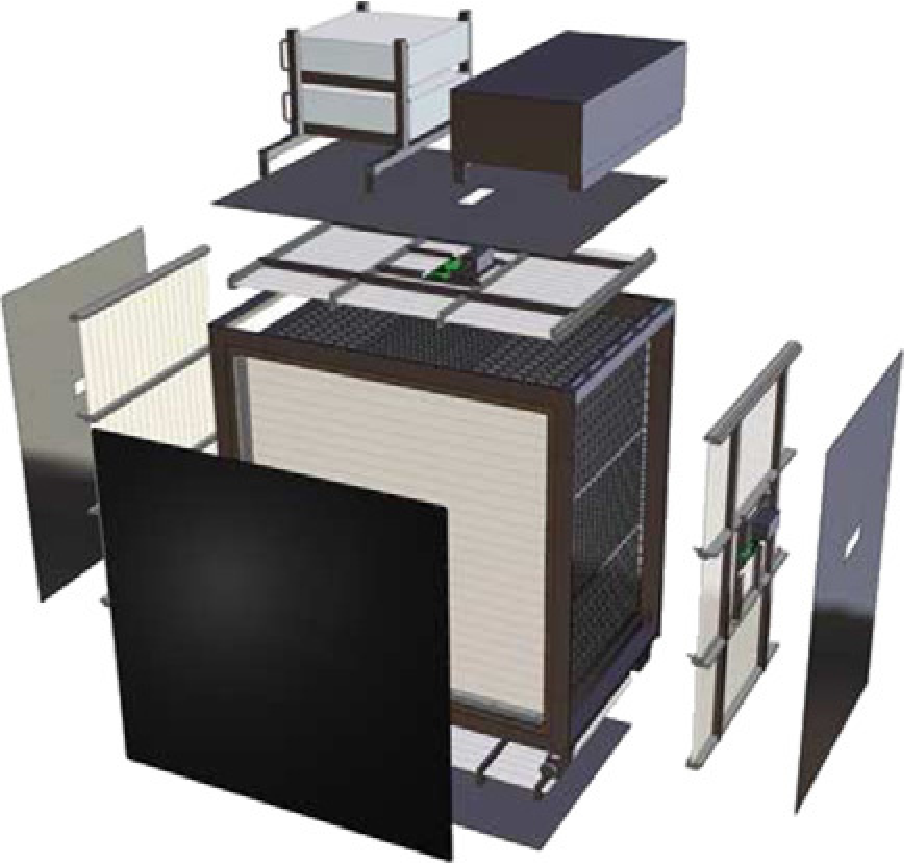
\includegraphics[width=0.5\linewidth]{fig/proton_module.pdf}
\end{center}
\caption{
Schematic view of INGRID Proton module.
}
\label{fig:proton_module}
\end{figure}


We will operate the INGRID Proton module using the T2K near detector electronics/DAQ system in the same way as J-PARC T59.
A proposal to use the module and its electronics for our project will be submitted to the T2K collaboration.

